\chapter{Methodology}
\label{ch:methodology}

\section{Research Model}
\label{sec:researchmodel}
	\begin{figure}[h]
		\centering
		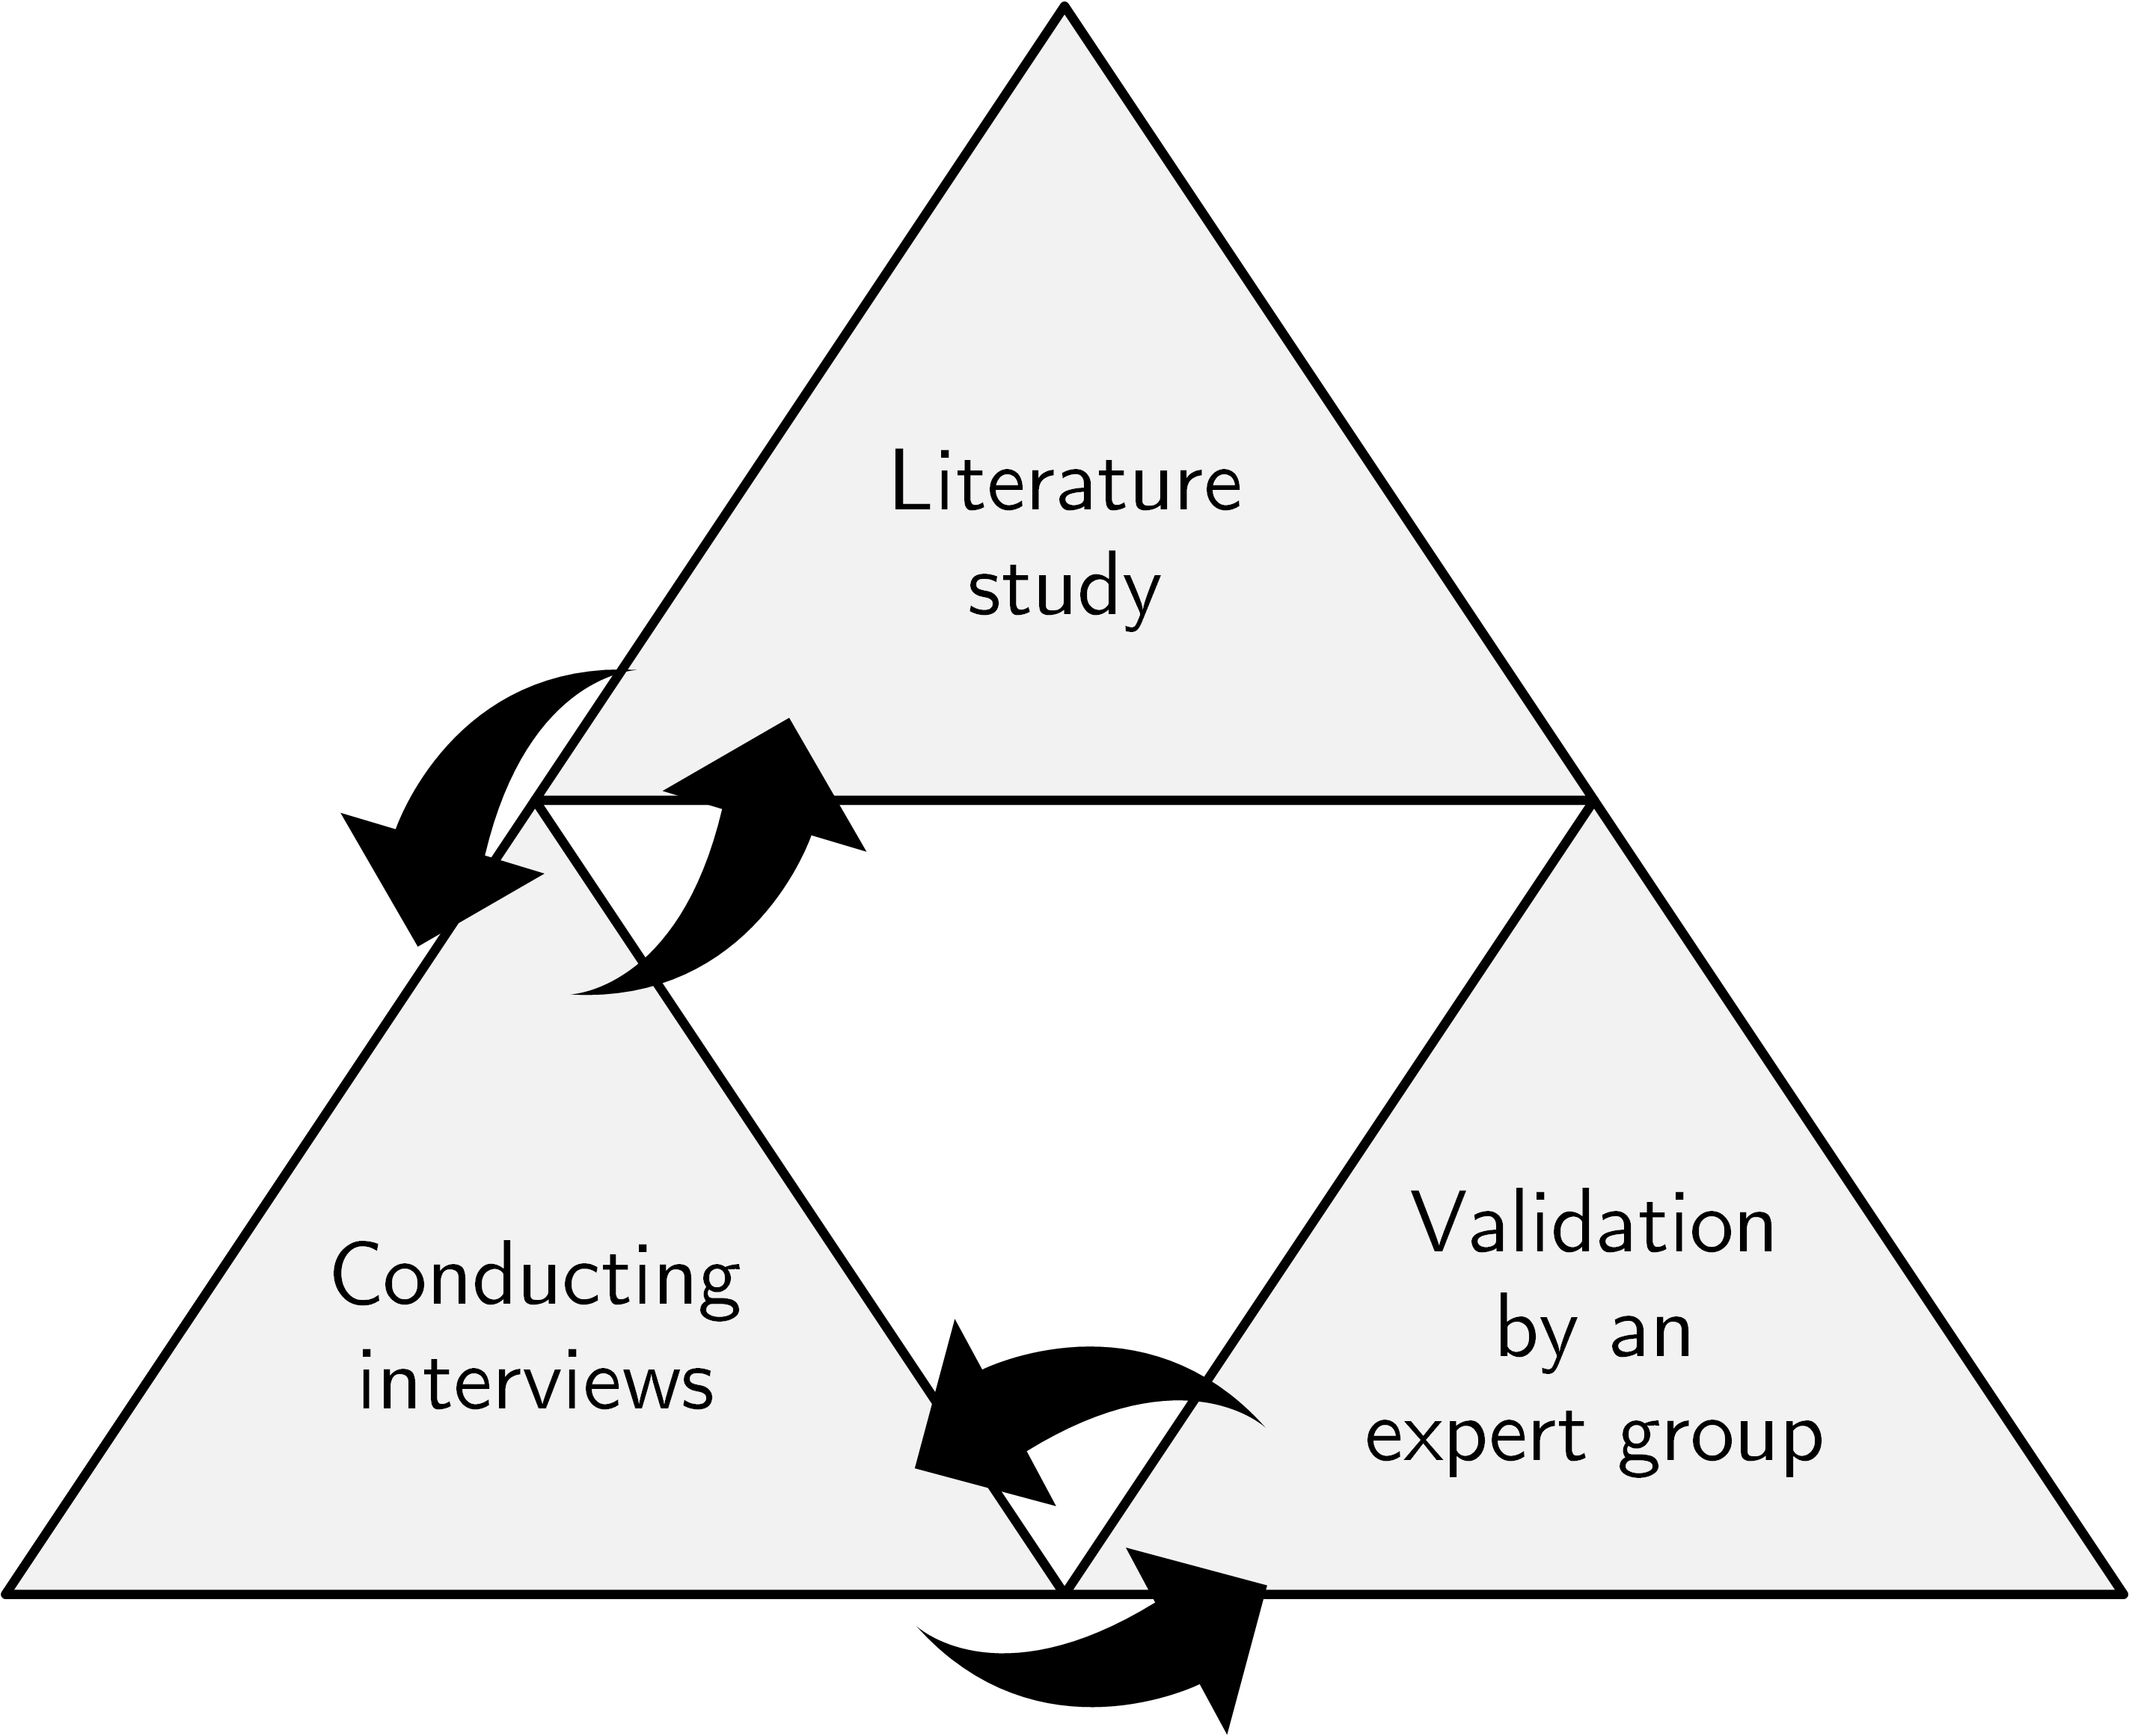
\includegraphics[width=14cm]{images/researchmodel}
		\caption[Research Model]{Research Model}
		\label{fig:research-model}
	\end{figure}

\section{Research quality}
\label{sec:researchquality}
The quality attributes of \textcite[p.~15--17]{Recker2013} are used to increase the rigorousness of the research. The quality attributes of \textcite[p.~15--17]{Recker2013} are supported by the \textit{\acrfull{osf}} of \textcite{Foster2017}, the \textit{\gls{fair}} of \textcite[Box 2]{Wilkinson2016}, and the application of \textit{Triangulation}, \cref{sub:triangulation}.

\subsection{Quality attributes}
\label{sub:qualityattributes}
\textcite[p. 15-17]{Recker2013} suggests using four attributes to increase the quality of research. The first attribute that is defined by \textcite[p.~15]{Recker2013} is \textit{Replicability}. \textcite[p.~15]{Recker2013} characterises \textit{Replicability} as the extend to which research procedures are repeatable. The attribute states that the procedures by which research outputs are created should be conducted and documented in a manner that allows others outside the research team to independently repeat the procedures and obtain similar, if not identical, results \parencite[p.~15]{Recker2013}. The second attribute stated by \textcite[p.~16]{Recker2013} is \textit{Independence} which is closely related to reliability. \textit{Independence} concerns the extent to which the research conduct is impartial and freed from any subjective judgment or other bias stemming from the researcher or research team itself \parencite[p.~16]{Recker2013}. \textit{Precision} is the third attribute defined by \textcite[p.~16]{Recker2013}. According to \textcite[p.~16]{Recker2013} \textit{Precision} states that in all scientific research the concepts, constructs, and measurements should be as carefully and precisely defined as possible to allow others to use, apply, and challenge the definitions, concepts, and results in their own work. The last attribute that \textcite[p.~16]{Recker2013} mentions is \textit{Falsification}. \textit{Falsification} describes the logical possibility than an assertion, hypothesis, or theory can be contradicted by an observation or other outcome of a scientific study or experiment \parencite[p.~16]{Recker2013}. The quality attributes are operationalised in this research as described in \cref{tab:operationalisationofqualityattributes}.
\begin{table}[!h]
	\centering
	\resizebox{\textwidth}{!}{%
	\begin{tabular}{p{.25\textwidth}p{.75\textwidth}}
		\toprule
		\textbf{Quality attribute} & \textbf{Operationalisation} \\%
		\midrule
		Replicability & \\%
		Independence & \\%
		Precision & \\%
		Falsification & \\%
		\bottomrule
	\end{tabular}
	}%
	\caption[Operationalisation of the quality attributes]{Operationalisation of the quality attributes}%
	\label{tab:operationalisationofqualityattributes}%
\end{table}
\subsection{The FAIR Guiding Principles}
\label{sub:fairguidingprinciples}
In \citeyear{Wilkinson2016} \citetitle{Wilkinson2016} was published in Scientific Data\footnote{\url{https://www.nature.com/sdata/}} by \citeauthor{Wilkinson2016}. \textcite[p.~3]{Wilkinson2016} emphasised \textit{FAIR}ness being applied to both human-driven and machine-driven activities. \textcite[Box 2]{Wilkinson2016} intended to provide guidelines to improve the Findability, Accessibility, Interoperability, and Reuse of digital assets. These principles are also called the \gls{fair}. The \gls{fair} describe distinct considerations for contemporary data publishing environments concerning supporting both manual and automated deposition, exploration, sharing, and reuse \textcite[p.~4]{Wilkinson2016}. The first step in (re)using data is to find it \parencite[p.~1]{GOFAIR2017}. According to \textcite[p.~1]{GOFAIR2017} metadata and data should be easy to find for both humans and computers. Machine-readable metadata is essential for the automatic discovery of datasets and services \parencite[p.~1]{GOFAIR2017}. \textit{Accessible} means that once the user finds the required data, it needs to know how it can be accessed \parencite[p.~1]{GOFAIR2017}. Accordingly to \textcite[p.~2]{GOFAIR2017} \textit{Interoperable} means that the data usually need to be integrated with other data. In addition, the data need to interoperate with applications or workflows for analysis, storage, and processing \parencite[p.~2]{GOFAIR2017}. The last guiding principle is stated by \textcite[p.~2]{GOFAIR2017} as \textit{Reusable}. Following \textcite[p.~2]{GOFAIR2017} the ultimate goal of the \gls{fair} is to optimise the reuse of data. Metadata and data should be well described so that they can be replicated and combined in different settings \parencite[p.~2]{GOFAIR2017}. The \gls{fair} are operationalised in the research as described in \cref{tab:fairguidingprincipilesoperationalised}.
\begin{table}[!h]
	\centering
	\resizebox{\textwidth}{!}{%
	\begin{tabular}{p{.25\linewidth}p{.75\linewidth}}
		\toprule
		\textbf{Guiding Principle} & \textbf{Operationalisation} \\
		\midrule
		Findable & The thesis, research, and data sets contain keywords, links, structures, and meta data that can be indexed. \\%
		Accessible & The thesis, research and data sets are published on GitHub, Zenodo, and Researchgate based on Open Access. Objects are created containing a location where the data can be acquired if it cannot be published because of author rights. \\%
		Interoperable & This principle is least relevant for this research. The data sets are qualitative based on literature, interviews, Expert Group feedback, and surveys. The created data sets are available for analysis and are stored in structured Microsoft Excel files. The files are easy to import or reuse in other environments. \\%
		Reusable & The publication of the thesis, research and data sets are licensed under a \href{https://creativecommons.org/licenses/by-sa/4.0/}{CC-BY-SA 4.0 license. The thesis, research, and data sets are allowed to be shared and adapted (commercially) as long as the original author is attributed and the possible derivate is published under the same license.} \\%
		\bottomrule
	\end{tabular}
	}%
	\caption[Operationalisation of the FAIR Guiding Principles]{Operationalisation of the FAIR Guiding Principles}%
	\label{tab:fairguidingprincipilesoperationalised}%
\end{table}

\subsection{The Open Science Framework}
\label{sub:osf}
One of the starting points of the research is Open Science. The idea behind Open Science is to allow scientific information, data and outputs to be more widely accessible (Open Access) and more reliably harnessed (Open Data) with the active engagement of all the stakeholders (Open to Society) \parencite{UNESCO2020}. The Center for Open Science\footnote{{\url{https://www.cos.io/}}} supports this way of research by supplying guidelines and even a toolkit. For this research the toolkit is used to support Open Access, Open Data and Open to Society. One of the tools in the toolkit is a reference model to select tools for the four main phases of research: Search and Discover, Design Study, Collect and Analyse Data, and Publish Reports. I use this reference model in section \ref{sec:researchinfraandtooling}. Using this framework will help in achieving replicability, precision, and reusability.

\begin{figure}[h!]
	\centering
	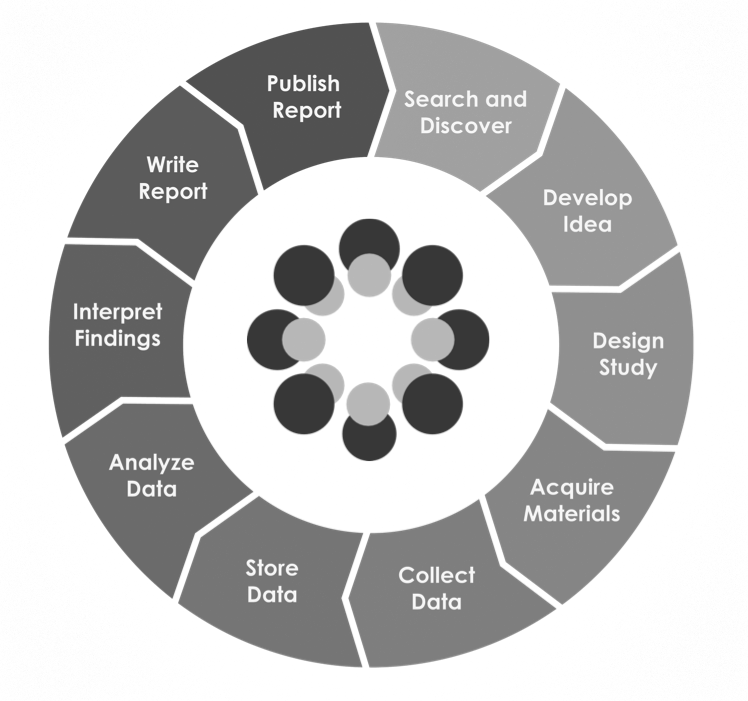
\includegraphics[width=0.5\linewidth]{images/osfbw}
	\caption[Open Science Framework]{Open Science Framework}
	\label{fig:openscienceframework}
\end{figure}

\subsection{Triangulation}
\label{sub:triangulation}
Triangulation has its origins in geography. To know the position of a distant object, two checkpoints are needed. The mutual distance between the calibration points and the angles relative to the object make it possible to calculate the correct distance via triangulation\footnote{\url{https://www.britannica.com/science/triangulation-trigonometry}} \parencite[p.~88]{Mortelmans2018}. Following \textcite[p.~88]{Recker2013} triangulation literally means doing more than just one thing \parencite[p.~88]{Recker2013}. According to \textcite[p.~110]{Recker2013} triangulation means you are seeking convergence and corroboration of results from different methods and designs studying the same phenomenon. Through triangulation, the researcher can gain a more nuanced picture of the situation and increase the reliability and validity of their findings \parencite[p.~88]{Recker2013}. \textcite[p.~88]{Recker2013} states that the use of triangulation assists researchers in increasing the robustness of results. Findings can be strengthened through the cross-validation achieved when different kinds and sources of data converge and are found to be congruent \parencite[p.~88]{Recker2013}. \textcite[p.~207]{Saunders2015} states that triangulation involves using more than one source of data and method of collection to confirm the validity, credibility, and authenticity of research data, analysis and interpretation. \textcite[p.~207]{Saunders2015} also stresses that it is a necessity to use \textit{triangulation} for a multi-method quantitative study, multi-method qualitative study or a mixed-methods study.

\textcite[p.~481]{Mortelmans2018} explains that in the qualitative research tradition, triangulation has become the method of choice for increasing the credibility of results. It is stated by \textcite[p.~481]{Mortelmans2018} that there are four types of triangulation. According to \textcite[p.~88]{Mortelmans2018} the first type is that of \textit{Data Triangulation}. \textcite[p.~481]{Mortelmans2018} states that with \textit{Data Triangulation}, different types of data are collected. The condition here is that the researcher stays within the qualitative paradigm \parencite[p.~481]{Mortelmans2018}. \textcite[p.~481]{Mortelmans2018} defines the second type \textit{Researcher Triangulation}. To avoid case contamination, multiple researchers analyse the same data \parencite[p.~482]{Mortelmans2018}. Afterwards, the results are compared with each other, and it is examined where any differences come from \parencite[p.~482]{Mortelmans2018}. The third case is defined by \textcite[p.~481]{Mortelmans2018} as \textit{Theory Triangulation}. \textcite[p.~482]{Mortelmans2018} explains that \textit{Theoretical Triangulation} means triangulating the results from different theoretical angles. Looking at data from a different perspective often yields compelling \parencite[p.~482]{Mortelmans2018}. The last type of triangulation is defined by \textcite[p.~481]{Mortelmans2018} as \textit{Methodological Triangulation}. According to \textcite[p.~483]{Mortelmans2018} explains \textit{Methodological Triangulation} as the combination of data collected by qualitative technique with data collected by quantitative means. However, \textcite[p.~483]{Mortelmans2018}\textit{Methodological Triangulation} explains it does not necessarily mean that quantitative methods are applied in research. 

\begin{figure}[h!]
	\centering
	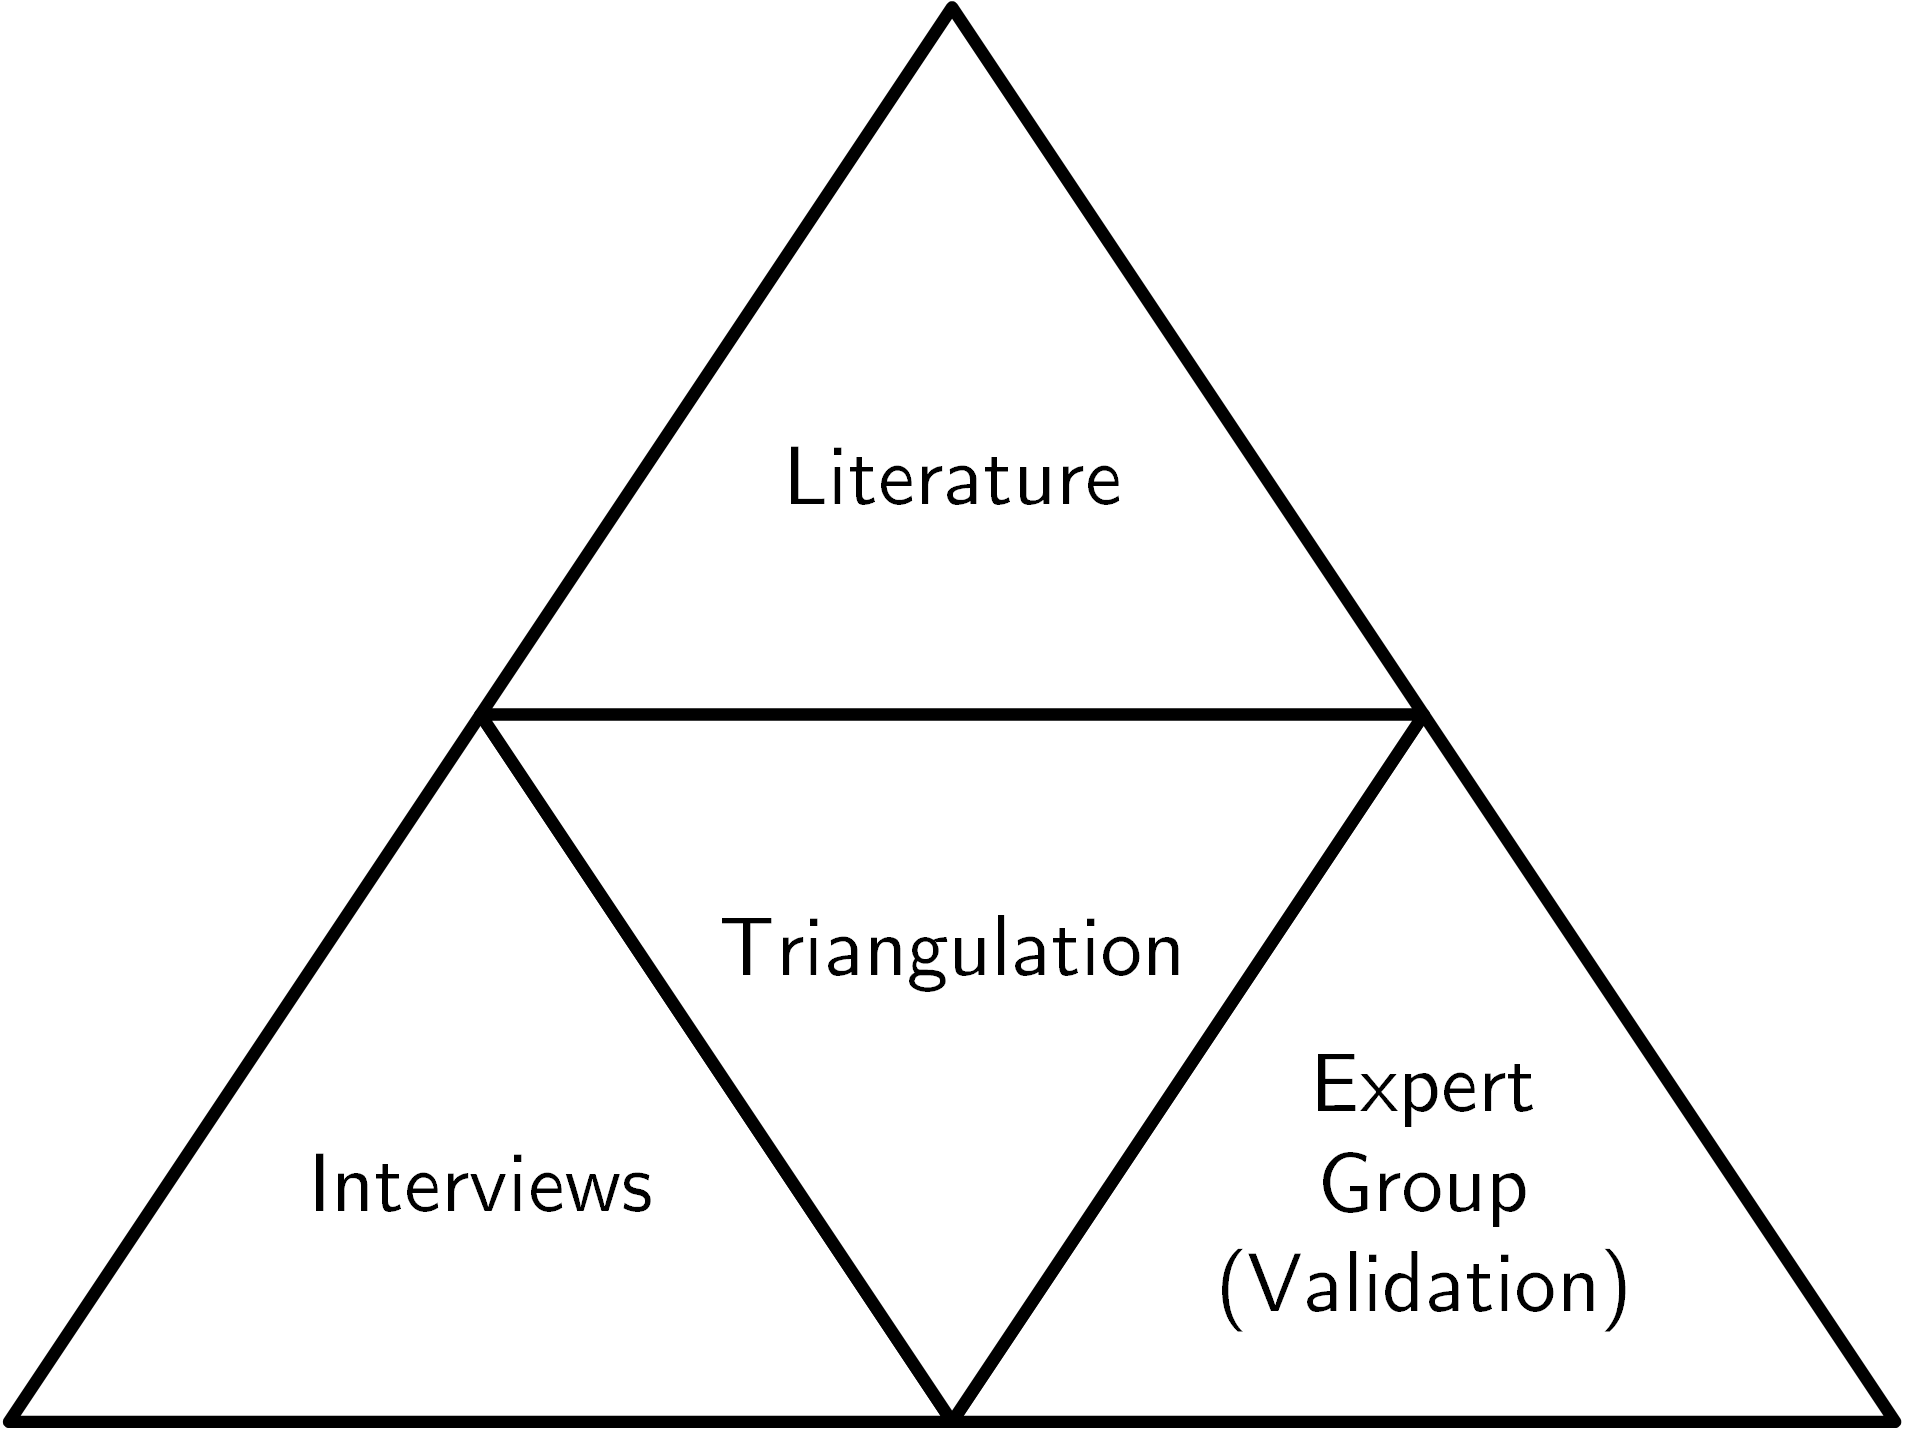
\includegraphics[width=0.5\linewidth]{images/triangulation}
	\caption[Operationalisation of Triangulation]{Operationalisation of Triangulation}
	\label{fig:triangulation}
\end{figure}

Triangulation is operationalised as Methodological Triangulation by using, as visualised by \cref{fig:triangulation}, literature study to abstract attributes, interviews with data analysis to validate attributes and an expert group with data analysis to validate attributes.

\section{Research approach}
\label{sec:researchapproach}
In this section, I describe the approach of the research. This description helps to increase replicability, independence, and reusability. For this research approach, I follow the research model (figure \ref{fig:research-model}) and the research (sub)questions (section \ref{sec:researchsubject}). The research model contains five phases in the research. The five phases are used to describe the research approach. The five phases are (a) Desk research, (b) Confrontation, (c) Analysis, (d) Validation, and (e) Conclusion and discussions.










\begin{table}[!h]
	\begin{center}
		\begin{tabular}{@{}ccccc@{}}
			\toprule
			EA/AF Success Factor & Literature & Delphi Group & Seen in Practice & Total \\ \midrule
			X    & 1    & 1   & 1   & 3   \\
			Y    & 1    & 1  & 0   & 2   \\
			Z    & 0    & 0   & 1   & 1   \\ \bottomrule
		\end{tabular}
		\caption{Example score triangulation}
		\label{tab:exampletriangulation}
	\end{center}
\end{table}

\begin{table}[!h]
	\begin{center}
		\begin{tabular}{@{}p{0.1\textwidth}p{0.9\textwidth}@{}}
			\toprule
			Score 	& Meaning of score \\ \midrule
			1		& It is not likely that it is an EA/AF success factor. \\
			2    	& It is somewhat likely that it is an EA/AF success factor. Additional research is required.\\
			3    	& It is likely that it is an EA/AF success factor. \\ \bottomrule
		\end{tabular}
		\caption{Meaning of the score of triangulation}
		\label{tab:exampletriangulationscoring}
	\end{center}
\end{table}

\begin{table}[!h]
	\begin{center}
		\begin{tabular}{p{0.2\textwidth}p{0.8\textwidth}}
			\toprule
			Score 	& Meaning of score \\ \midrule
			1		& There is no sure indication of an EA/AF Success Factor. \\
			2    	& There is, with some certainty, an indication for an EA/AF Success Factor. Additional research is required to validate the EA/AF Success Factor. \\
			3    	& There is undoubtedly an indication of an EA/AF Success Factor. \\ \bottomrule
		\end{tabular}
		\caption{Meaning of the score of triangulation}
		\label{tab:oldexampletriangulationscoring}
	\end{center}
\end{table}


\subsection{Desk research}
\label{sub:deskresearchphase}
The first phase of the research model emphasises desk research on the relevant concepts, theories and definitions. Desk research is conducted based on a literature study. The main concepts of \gls{antifragile}, \acrshort{ea}, \acrshort{vuca}, and the public sector are studied. This first phase (a) will answer the sub-questions of:
\begin{itemize}
	\item{What is literature saying about \gls{antifragile}?}
	\item{What is literature saying about the public sector?}
	\item{What is literature saying about \acrlong{ea}?}
	\item{What is literature saying about the success factors of Enterprise Architecture?}
\end{itemize}

\subsubsection{Literature research}
For the literature research two primary methods are used. The first method is (foward and backward) snowballing of already acquired literature. The second method is the use of online scientific libraries.

\begin{figure}[H]
	\centering
	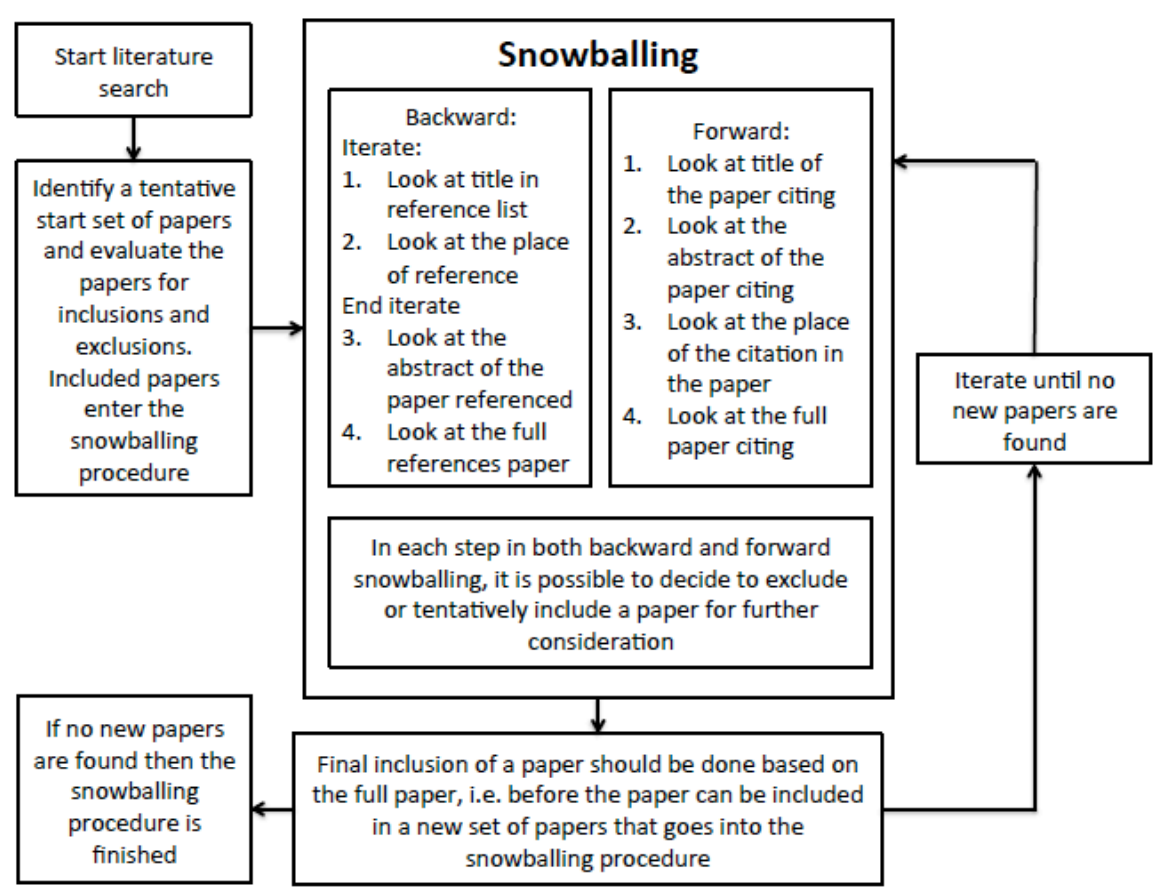
\includegraphics[width=0.6\linewidth]{images/snowball}
	\caption[Snowballing literature]{Snowballing literature \parencite{Wohlin2014}}
	\label{fig:snowball}
\end{figure}
For finding relevant literature online scientific libraries are used. The online scientific libraries are Web of Science, Research Gate, and Google Scholar. The full concept name is used and the known abbreviations of the concept (e.g. Enterprise Architecture and EA). The list of abbreviations contains the used abbreviations. Literature is only accepted if the literature complies with quality attributes. These attributes are accuracy, authority, objectivity, currency, and coverage\footnote{\url{https://libguides.library.cityu.edu.hk/litreview/evaluating-sources/}}. All found literature is administrated for replicability, independence, precision, accessibility, and reusability. Section \ref{sub:tbresearchexecution} describes how literature registration and administration is executed.

\subsubsection{Antifragile}
\label{subsub:antifragile}
The literature study on \gls{antifragile} makes use of four primary sources. The first primary source is the book ''\Gls{antifragile}: Things that gain from disorder'' \parencite{Taleb2012}. \textcite{Taleb2012} is the progenitor of the \gls{antifragile} theory. The second primary source is the master thesis ''Defining \Gls{antifragility} and the application on Organisation Design" \parencite{Botjes2020}. \citeauthor{Botjes2020} studied the literature, extensively, in the field of \gls{antifragile} and the application in the context of an organisation. By using the thesis of \citeauthor{Botjes2020} the literature study of this study concentrates on the literature after 2018. The last two primary resources are the articles ''No More Snake Oil: Architecting \Gls{agility} through \Gls{antifragility}'' and ''The Philosophy of Residuality Theory'' \parencite{OReilly2019,OReilly2021}. \textcite{Botjes2020} did not use the articles of \citeauthor{OReilly2019}. The theories of \citeauthor{OReilly2019} were less of interest for the subject of \citeauthor{Botjes2020}. While for this research the Residuality Theory of \textcite{OReilly2021} has added value since it targets system architecture.

\begin{remark}
	Need to add second book from Taleb (Black Swan) since Antifragile is an answer to black swan events.\\
	Need to add book of Hole as it is one of the sources referenced by many.
\end{remark}

The first method for literature study is snowballing. Snowballing of these sources is used to determine other important literature on \gls{antifragile}. Forward snowballing is used for the source of \citeauthor{Taleb2012}. Since \citeauthor{Taleb2012} is the progenitor, it is not necessary to do a backward snowballing. Backward snowballing is used for the sources from \citeauthor{Botjes2020} and \citeauthor{OReilly2019}.

The second method for literature study is the use of online scientific libraries. For these libraries the following set of keywords or key sentences are used.
\bigskip

\begin{table}[H]
	\centering
\begin{tabular}{p{0.4\textwidth}p{0.4\textwidth}}
	\toprule
	\gls{antifragile}	& \gls{antifragile} \gls{robust} \gls{resilient} \gls{agile}\\%
	\gls{antifragile} \acrlong{ea}	& \gls{antifragile} public sector\\%
	\gls{antifragile} success factors & residuality theory\\%
	\gls{antifragile} residuality theory & \acrlong{vuca} \\%
	\gls{antifragile} system & \\%
	\bottomrule
\end{tabular}
	\caption{Antifragile keywords}
	\label{tab:antifragilekeywords}
\end{table}

\subsubsection{Enterprise Architecture}
\label{subsub:enterprisearchitecture}
As described earlier in the subsection \ref{sub:eathreeschools} the definition of the \acrfull{ea} school of \acrfull{eea} is the school that fits in with \gls{antifragility}. \textcite[p. 42]{Lapalme2012} states that there are seven dominant authors in the school of \acrshort{eea}.  The literature study on \acrshort{ea} will focus on these authors. These authors are:

\begin{table}[H]
	\centering
	\begin{tabular}{p{0.4\textwidth}p{0.4\textwidth}}
		\toprule
		Jamshid Gharajedaghi & Tom Graves \\%
		Jan Hoogervorst	& James Martin \\%
		Kevin Smith & James Lapalme\\%
		Donald de Guerre &  \\%
		\bottomrule
	\end{tabular}
	\caption{\acrshort{eea} authors}
	\label{tab:eeaauthors}
\end{table}

The book of \textcite{Hoogervorst2009a} on Enterprise Governance and Enterprise Engineering, and \textcite{Lapalme2012} on the three schools of \acrshort{ea} are used as a starting point of the literature study. 

The first method is snowballing. The two sources will be used for forward and backward snowballing. The second method for literature study is the use of online scientific libraries. For these libraries the following set of keywords and key sentences are used:

\begin{table}[H]
	\centering
\begin{tabular}{p{0.4\textwidth}p{0.4\textwidth}}
	\toprule
	\acrlong{ea} & \acrlong{ea} sucess factors\\%
	\acrlong{ea} \gls{antifragile} system	& \acrlong{ea} steering mechanism\\%
	intentional emergent \acrlong{ea} & \acrlong{ea} Business Strategy\\%
	\acrlong{ea} public sector & \acrlong{ea} system-in-environment \\%
	\bottomrule
\end{tabular}
	\caption{Enterprise Architecture keywords}
	\label{tab:enterprisearchitecturekeywords}
\end{table}

\subsubsection{Public sector}
\label{subsub:publicsector}
The literature study on public sector makes use of one primary source. \textcite{Wal2008} is an article on the differences between the public and private sector based on the core values of these sectors. This article is used for forward and backward snowballing. The last method for literature study is the use of online scientific libraries. For these libraries the following set of keywords and key sentences are used:

\begin{table}[H]
	\centering
	\begin{tabular}{p{0.4\textwidth}p{0.4\textwidth}}
		\toprule
		Difference public and private sector &	public sector \gls{antifragile}\\%
		Collaboration public and private sector & public sector \gls{resilient}\\%
		public sector \acrshort{vuca} & \\%
		\bottomrule
	\end{tabular}
	\caption{Public sector keywords}
	\label{tab:publicsectorkeywords}
\end{table}

\begin{remark}
	The preliminary research on the topic public sector is not started yet. Maybe some primary sources will emerge.
\end{remark}

\subsection{Confrontation}
\label{sub:confrontationphase}

For the confrontation of VUCA with the public sector interviews are used to....\\
For the confrontation of EA with EA a framework/model is needed! (part of Theoretical background)

\begin{remark}
	What is the model for confrontation?
	I have to determine the lens I am going to use.
\end{remark}

The second phase (b) 

\subsection{Analysis}
\label{sub:analysisphase}

\begin{remark}
	What is the model for Analysis?
	I have to determine the lens I am going to use.
\end{remark}

The third phase (c)

How can the success factors of \acrlong{ea} contribute to becoming antifragile?

\subsection{Validation}
\label{sub:validatinphase}
%The fourth phase (d) analyses the outcome of the analysis phase. This outcome is the answer to the sub-question ''How can the success factors of \acrlong{ea} contribute to becoming antifragile?'' 
The success factors are validated by the means of the Delphi Method.

\subsubsection{Delphi Method}
\label{subsub:delphimethod}
The Delphi method is an iterative process to collect and distil the anonymous judgments of experts using a series of data collection and analysis techniques interspersed with feedback. The Delphi method is well suited as a research instrument when incomplete knowledge about a problem or phenomenon. The Delphi method evolved into a flexible research method appropriate for many \acrfull{is} research projects, such as determining the criteria for \acrshort{is} prototyping decisions, ranking technology management issues in new product development projects, and developing a descriptive framework of knowledge manipulation
activities. The Delphi method is a flexible, effective and efficient research method that can be successfully used by \acrshort{is} graduate students to answer research questions in \acrshort{is} and to advance the \acrshort{is} Body of Knowledge rigorously. \parencite{Skulmoski2007}

The group participants are mutually unknown, I am the only one who knows who the participants are. When it cannot be proven that the artefact is incorrect, it must be correct. This method is the principle of falsification. To reach a consensus, I use questionnaires. To reach a consensus, I am working iterative and adjusts the artefact after the feedback. I expect consensus on the artefact after two to six rounds of questionnaires. The goal of the Delphi Rounds is that it cannot be proven that the sucess factors are incorrect. This method is the principle of falsification (subsection \ref{sub:recker}). However, when is there a consensus? \textcite[p. 404]{Diamond2014} concludes in his research for over more than 100 cases that the median of the percentage of consensus 75\% is. I state, as a result of the research of \textcite{Diamond2014}, that consensus is reached with the threshold of 75\%. I state with some degree of certainty that the artefact is correct with a consensus of 75\%.

I defined domains for the group composition based on the context of the research. These domains are \acrfull{isv}, Municipality, National Government, VNG-Realisatie (the association of Dutch municipalities), and Academics. Participants are members of one or more of these domains and have an affinity with Enterprise Architecture and the public sector. I invite at least three participants per domain (n=3). The result is a total population of at least fifteen (n=15). The approach followed \textcite{Denzin2017} multiple triangulation approach, which encourages several methods to collect data and multiple investigators with varied expertise.

For the Delphi Group composition domains are defined based on the context of the research. These domains are \acrfull{isv}, Municipality, National Government, VNG-Realisatie (the association of Dutch municipalities), and Academics. The participants have affinity with \acrshort{ea}. The participants validate the artefact their context and domain.

Meeting Wizard is the service for sending out the questionnaires and execute the analysis of the outcome of the questionnaires. The participants get an invite by email to fill in the questionnaires. I analyse the results after every round and communicates the outcome as soon as a consensus is reached.

\subsection{Conclusion and discussion phase}
\label{sub:conclusionanddiscussinophase}
The fifth phase (e)

What are the success factors of \acrlong{ea} for \gls{antifragility} in the public Sector?

\section{Research type}

\begin{remark}
	Qualitative vs Quantitative! (use \parencite{Recker2013})
\end{remark}


\section{Research infrastructure and tooling}
\label{sec:researchinfraandtooling}
\begin{wrapfigure}{R}{0.5\textwidth}
	\begin{center}
		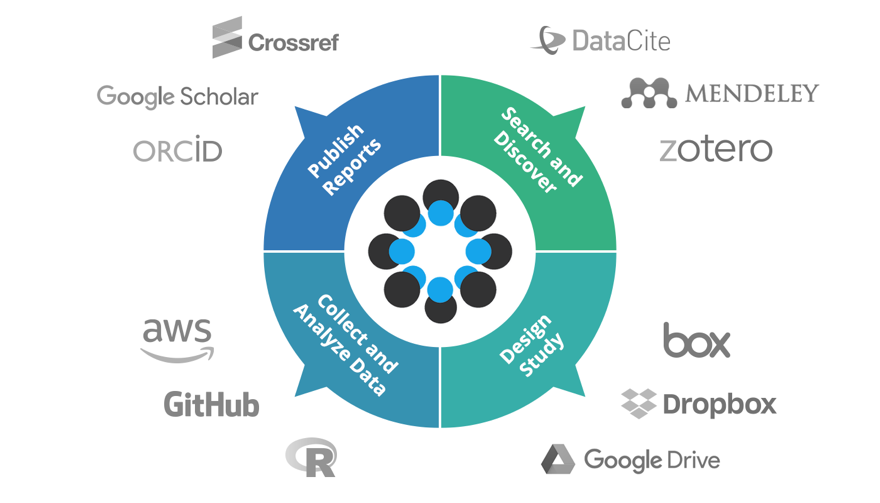
\includegraphics[width=0.5\linewidth]{images/osfframework}
		\caption[Open Science Framework]{Open Science Framework}
		\label{fig:osfframework}
	\end{center}
\end{wrapfigure}
For selecting the suitable instruments for the research, the Open Science Framework\footnote{\url{https://www.cos.io/products/osf}} is used. The Open Science Framework consists out of 4 stages in a research project. Those stages are: ''Search and Discover, Design Study, Collect and Analyse, and Publish Reports.'' The Open Science Framework proposes specific infrastructure and tools per stage. The transparency in the used infrastructure and tools increases the quality of the research. It increases the replication factor, findability, accessibility, interoperability, and reusability.
\subsection{Thesis creation}
\label{sub:tbresearchcreation}
I used my corporate laptop (Dell Latitude 7200 2-in-1\footnote{\url{https://www.dell.com/en-us/work/shop/dell-laptops-and-notebooks/latitude-7200-2-in-1-laptop/spd/latitude-12-7200-2-in-1-laptop}}) with Windows 10 Professional installed for creating the thesis. The thesis is created with the markup language \LaTeX\footnote{\url{https://www.latex-project.org/}}. The used typesetting environment is TexLive\footnote{\url{https://www.tug.org/texlive/}} with the document type of ''Report'' from KOMA-Script\footnote{\url{https://ctan.org/pkg/koma-script}}. TexStudio\footnote{\url{https://www.texstudio.org/}} is the used \LaTeX\ Editor. It supports syntax-highlighting, has an integrated viewer, reference checking and numerous wizards. For the creation and administration of references Bib\LaTeX\footnote{\url{https://ctan.org/pkg/biblatex/}} is used with the reference manager JabRef\footnote{\url{https://www.jabref.org/}} with the citation style of APA 7th Edition\footnote{\url{https://apastyle.apa.org/}} and with web browser integration. The files are stored on a personal Dropbox\footnote{\url{https://www.dropbox.com/}} that is used by GitHub Desktop\footnote{\url{https://desktop.github.com/}} to synchronise with a public GitHub repository\footnote{\url{https://github.com/JRBliekendaal/master-thesis}}. GitHub\footnote{\url{https://github.com/}} is used for source control but also for reviewing and discussing the topics with the (Co-)Promotor and the planning of the master thesis project. The thesis source files are copied to an Amazon S3 Blob\footnote{\url{https://aws.amazon.com/s3/}} for backup. The backup rotation is seven versions. Cloudberry Explorer Freeware for Amazon S3\footnote{\url{https://www.msp360.com/explorer/windows/amazon-s3.aspx}} is used for backup. Grammarly\footnote{\url{https://www.grammarly.com}}, with the paid subscription service, checks the thesis for spelling, grammar,  style, and plagiarism. The used goals for Grammarly are audience=knowledgeable, formality=formal, and domain=academic. Microsoft Visio Professional\footnote{\url{https://www.microsoft.com/en-ww/microsoft-365/visio/}} is used to create figures. The GitHub repository contains all the sources.
\subsection{Research administration}
\label{sub:tbresearchadministration}
The research administration, which includes documentation containing privacy-sensitive information, like the name and contact information of the Delphi Group participants, is stored on a non-public GitHub Repository\footnote{\url{https://github.com/JRBliekendaal/master-thesis-administration}}. The private GitHub Repository is also for staging thesis parts that still need to be anonymised. For taking notes Leuchtturm1917\footnote{\url{https://www.leuchtturm1917.us/notebook-classic.html}} Notebooks are used with mechanical pencils of Faber-Castell\footnote{\url{https://www.fabercastell.com/products/tk-fine-vario-l-mechanical-pencil-10mm-135900}} and pens from Sakura\footnote{\url{https://www.sakuraofamerica.com/product/pigma-micron/}} with long-lasting ink.
\subsection{Research execution}
\label{sub:tbresearchexecution}
For the execution of the research, Microsoft Excel\footnote{\url{https://www.microsoft.com/en-us/microsoft-365/excel}} is used for the administration of the literature research. For the administration of the literature research, the following headers are used: ID (for a unique ID per item), search terms used, scope, title, subtitle, author(s), year, type, Bib\LaTeX\ citation key, title relevance, abstract relevance, content relevance, found at, doi/isbn, url, date found, duplicate, date used, use for, and notes. Researchgate\footnote{\url{https://www.researchgate.net/}}, Web of Science\footnote{\url{https://app.webofknowledge.com/}}, and Google Scholar\footnote{\url{https://scholar.google.com/}} are the main sources for searching for literature. PaperPanda\footnote{\url{https://paperpanda.app/}} is used for hard to find literature. The literature administration is, together with the publicly available literature, stored in the repository of the master thesis. For non-public available literature, the administration contains the location where the literature is retrievable. All the literature is added to a bib\LaTeX\ file for future reference. For traceability the entries in the bib\LaTeX\ file contain the Unique ID in the notes field. JabRef is used to sort the references by using subgroups to support the workflow. The subgroups used are: ''evaluate, rejected, and used.'' Only the literature in the subgroup used are transferred to the bibliography file of the thesis. This prevents cluttering. For working as paperless as possible all the literature, where possible, is in pdf or in ebook format. For reading Acrobat Reader DC\footnote{\url{https://get.adobe.com/reader/}} is used for reading the PDF, and an Amazon Kindle Oasis\footnote{\url{https://www.amazon.com/dp/B07L5GJD99}} for eBooks. With the Amazon Kindle the highlight feature is used. This is not stored on GitHub since the highlights are under copyright of the author(s).\par
For the execution of the Delphi Method, Meetingwizard\footnote{\url{https://www.meetingwizard.nl/}} is used for questionnaires and the analysis of the questionnaires. The license for using Meeting Wizard is supplied by the Antwerp Management School.

\subsection{Summary of used infrastructure and tooling}

\begin{table}[!h]
	\begin{center}
		\begin{tabular}{@{}cccc@{}}
			\toprule
			\textbf{Search \& Discover} & \textbf{Design Study} & \textbf{Collect \& Analyse Data} & \textbf{Publish Reports}\\ \midrule
			Web of Science & 1    & JabRef   & \LaTeX \\%
			ResearchGate   &      &           & TeXstudio \\%
			Google Scholar & 2    & PaperPanda  & ORCID \\%
			Z	 & 0    & bib\LaTeX   & ResearchGate \\%
			Z	 &	x	& Meetingwizard	  & Zenodo \\%
			Z	 &	x	& Microsoft Excel  & Grammarly \\%
			Y    & 2    & GitHub  & Microsoft Visio \\%
			Y	 & 2	& Cloud Berry Explorer for S3 & \\%
			Y	&	&	QDA Miner Lite & \\%
			\bottomrule
		\end{tabular}
		\caption{Used infrastructure \& tooling}
		\label{tab:usedinfrastructuretooling}
	\end{center}
\end{table}